% Top-level LaTeX file
%
% Book template authors: Jeff C. Jensen, Edward A. Lee, and Sanjit A. Seshia.
% Derived from Lee & Seshia: Embedded Systems, A Cyber-Physical Systems Approach.
%
% Solutions mode is set by boolean parameters below.
%
% To build a PDF:
%   make
%
% To clean:
%   make clean

\documentclass[pdftex,11pt,openany,oneside]{book}
% preamble

% Indicate that PDF v1.6 or earlier may be included in figures
\pdfoptionpdfminorversion 6

% nag user if including deprecated packages
\RequirePackage[l2tabu, orthodox]{nag}

% iPad screen is 1024x768, 9.7 inch diagonal. Dimensions:
% Width: 0.007578125*768=5.82
% Height: 0.007578125*1024=7.76
% Scale this up by 1.064 to get slightly smaller fonts.
% Width: 6.19
% Height: 8.25
\usepackage[papersize={6.19in, 8.25in},top=0.6in,bottom=0.6in,left=0.4in,right=0.4in]{geometry}

% MicroType package to improve "glue" and reduce hbox & vbox fill problems
\usepackage{microtype}

% Paragraph spacing and style
\parskip        0.1in
\parindent      0.0in

% Packages
\usepackage[margin=10pt,font=small,labelfont=bf]{caption}
\usepackage{graphicx}
% To get decent pdf files:
\usepackage{mathptmx} % Use Times as default text font, and provide maths support
\usepackage{amsmath}
\usepackage{amsfonts}
\usepackage{amssymb}
\usepackage{ifthen}
\usepackage{color}
\usepackage[usenames,dvipsnames]{xcolor} % for color names
\usepackage{boxedminipage}
% To have floating figures
\usepackage{floatflt}
% To have subfigures
\usepackage{subfigure}
% To span rows in a table:
\usepackage{multirow}
% To allow paragraphs aligned at the bottom in a table.
\usepackage{array}
% To get a decent bibliography:
\usepackage{natbib}
% To get section headings in helvetica.
%   OT1: text font
%   phv: Adobe Helvetica
%   b: bold (alt: bc: bold condensed)
%   n: normal (not italic (i) or small caps (sc) etc.)
\usepackage{sectsty}
\allsectionsfont{\usefont{OT1}{phv}{b}{n}\selectfont}
% To get fancy chapter headings (must be after sectsty package)
\usepackage[Bjornstrup]{fncychap}
\ChTitleVar{\raggedleft\Huge\bfseries}
% frames for solutions environment
\usepackage{tcolorbox}
\tcbuselibrary{breakable}
\tcbuselibrary{skins}
% For more compact table of contents.
% NOTE: setspace package conflicts with hyperref and causes footnotes
% to hyperlink to page i, for some strange reason. Putting it before hyperref
% seems to solve the problem.
\usepackage{setspace}
% To penalize widows
\widowpenalty=10000
\clubpenalty=10000
% Use the version package
\usepackage{version}
% For code listings
\usepackage{listings}
% for compact enumerations
\usepackage{paralist}

\usepackage{xstring}  % for \StrSubstitute, used for \menulist
\usepackage{microtype} % better hyphenation and line breaking for \texttt \ttfamily
\usepackage{fancybox}  % for enclosed ovalbox

% For indexing
\usepackage{makeidx}
\makeindex

\usepackage{algorithm,algorithmic}
\usepackage[algo2e,lined,linesnumbered,algochapter]{algorithm2e}

%fonts and encoding
% use T1 encoding for special characters (pipes, backslashes, etc.)
\usepackage[T1]{fontenc}
% load symbol definitions
\usepackage{textcomp} % for textregistered, texttrademark, etc.
% make underscore a text character unless in math mode
\catcode`_=12
\begingroup\lccode`~=`_\lowercase{\endgroup\let~\sb}
\mathcode`_="8000
% for external link symbol
\usepackage{MnSymbol}
% for \dsliterary symbol for document links
\usepackage{dictsym}
% for \makefirstuc
\usepackage{mfirstuc}

% Hyperlinks
\usepackage{hyperref}
% To ensure that hyperlinks to figures, etc., show the entire figure when you go to them.
% Note that this requires that every \begin{figure}...\end{figure} have a \caption.
\usepackage[figure,table]{hypcap}
% Add additional PDF metadata to PDF file by including this package
\usepackage{hyperxmp}

% To enable file writing
\usepackage{catchfile}

% Use for key pairings
\usepackage{pgfkeys}

% For getting the full page titlepage.
\usepackage[absolute]{textpos}

% allow inclusion of external PDF pages
\usepackage{pdfpages}

% Headers and footers
\setlength{\headheight}{14pt}
\usepackage{fancyhdr}
% Bug in fancyhdr results in overfull hbox beyond margin (offset chapter number)
% fix this here by kerning -10pt (the amount of overfill)
\makeatletter
  \renewcommand{\DOCH}{%
    \settowidth{\py}{\CNoV\thechapter}%
    \addtolength{\py}{-10pt}%     % Amount of space by which the
%                                  % number is shifted right
    \fboxsep=0pt%
    \colorbox[gray]{.85}{\rule{0pt}{40pt}\parbox[b]{\textwidth}{\hfill}}%
\kern-\myhi
    \kern-\py\raise20pt%
    \hbox{\color[gray]{.5}\CNoV\thechapter}%
%\kern-\myhi
\\%
  }
\makeatother


%%%%%%%%%%%%%%%%%%%%%%%%%%%%%%%%%%%%%%%%%%%%
% Files input or output by this document   %
%%%%%%%%%%%%%%%%%%%%%%%%%%%%%%%%%%%%%%%%%%%%
% Filename of the .bib file to generate for external references; omit extension
\newcommand{\referencesexternal}{references-external}

%%%%%%%%%%%%%%%%%%%%%%%%%%%%%%%%%%%%%%%%%%%%
% Release settings                         %
%%%%%%%%%%%%%%%%%%%%%%%%%%%%%%%%%%%%%%%%%%%%
% Version number of this release
\newcommand\releaseversion{1.0}
% Location of PDFs that should be distributed with this document
\newcommand\docpath{file:documents}

% Release settings: draft and solution.
%
%% To print solutions, set this value to true
\newboolean{SOLUTIONS}
\setboolean{SOLUTIONS}{true}
%% To print FIXME messages, set this value to true
\newboolean{DRAFT}
\setboolean{DRAFT}{true}

\title{Book Title}
\author{First Author \and Second Author \and Third Author}

% License statement and URL are used in the title page, as well as
% the \hypersetup PDF options
\newcommand\license{Copyright \copyright YYYY, AUTHORS. All rights reserved. This textbook and supplemental material are licensed under LICENSE (SHARING IS CARING!).}

% Setup hyperlink appearance.
\definecolor{linkColor}{rgb}{0.1,0.1,0.8}
\hypersetup{
    colorlinks=true,
    linkcolor=linkColor,
    citecolor=linkColor,
    urlcolor=linkColor,
    filecolor=linkColor,
    plainpages=false,
    linktocpage=true,
    breaklinks=true,
    pdfnewwindow=true,
    pdfpagemode=UseOutlines,
    pdfcopyright=\license
}

%%%%%%%%%%%%%%%%%%%%%%%%%%%%%%%%%%%%%
% The document
%%%%%%%%%%%%%%%%%%%%%%%%%%%%%%%%%%%%%

\begin{document}
% Commands and environments
% Authors: Jeff C. Jensen, Edward A. Lee and Sanjit A. Seshia
% Date: 2016-06-08
% Copyright: (c) 2016, all rights reserved.
% License: Creative Commons Attribution 4.0 International (CC BY 4.0).

% File writing commands

% \appendwrite{filename}{content}
\newwrite\appendwrite
\newcommand\appendfile[2]{
    \begingroup
    \IfFileExists{#1}
        {\CatchFileDef{\filecontent}{#1}{\endlinechar=`^^J\catcode\endlinechar=12\relax}}% keep existing end-of-lines
        {\let\filecontent\empty}%
    \createfile{#1}{\filecontent#2}
    \endgroup
}

% create (overwrite) a new file
% \createfile{filename}{content}
\newwrite\createwrite
\newcommand\createfile[2]{
    \immediate\openout\createwrite=#1
    \immediate\write\createwrite{#2}
    \immediate\closeout\createwrite
}

% Authors: Jeff C. Jensen, Edward A. Lee and Sanjit A. Seshia
% Date: 2016-06-08
% Copyright: (c) 2016, all rights reserved.
% License: Creative Commons Attribution 4.0 International (CC BY 4.0).

%%%%%%%%%%%%%%%%%%%%%%%
% References          %
%%%%%%%%%%%%%%%%%%%%%%%
%
% This document enables efficient and consistent management of references, citations,
% external URLs, and PDF documents distributed with this text.
%
% Some commands create BiBTeX entries and associate them to file paths or URLs. The
% bibliography label, BiBTeX entry, and PDF filename or URL are defined in a single
% command and referenced similarly. This addresses the problem of connecting BiBTeX,
% PDFs, and URLs when printing a citation. Without this framework, each citation
% requires a hard-coded link to a PDF document or a URL and must be followed by the
% corresponding BiBTeX citation. For example, consider:
%
%    \link{doc.pdf}{Doc Title}~\cite[]{Authors:Year:Title}
%
% If a PDF is updated to a new version, or a URL changes, or the year is updated,
% then every instance of the PDF link and BiBTeX label reference must be changed, and
% the PDF must be in the correct location in the filesystem. This is too complex a
% way to manage dozens of such references.
%
% For references into external PDFs distributed with this document, one command
% creates a BiBTeX entry, verifies the document exists in the distribution, and
% associates the citation with a file path. A complementary citation command
% prints a text citation with the appropriate link to the PDF file and link to the
% bibliography entry.
%
% For references into external URLs, one command creates a BiBTeX entry and associates
% the citation with a URL. A complementary citation command prints a text vitation
% with the appropriate URL link and link to the bibliography entry.
%
% Use Case:
%   Internal (this document) references
% Syntax:
%   \chapref{label}                                   for Chapter 1: ChapTitle
%   \secref{label}                                    for S1.2.3 (SecTitle)
%   \sideref{label}{sidetitle}                        for 'sidetitle' sidebar p.{label}
%   \exref{label1,...}                                for Ex. #1,...
%   \chapsecref{chaplabel}{seclabel}                  for Chapter 1: ChapTitle, S1.2.3 (SecTitle)
%   \chapsideref{chaplabel}{sidebarlabel}{sidetitle}  for Chapter 1: ChapTitle, ``SideTitle'' sidebar p.1
%   \chapexref{chaplabel}{exlabel1,...}               for Chapter 1: ChapTitle, Ex. #1,...
%   \chapsecexref{chaplabel}{seclabel}{exlabel1,...}  for Chapter 1: ChapTitle, S1.2.3 Ex #1,...
%   \labref{label}                                    for Lab 1: LabTitle
% Examples:
%   Refer to \secref{lab:eclipseTroubleshooting} for troubleshooting Eclipse.
%   This lab builds on \labref{lab:ProgramMicroBlazeXilinx}.
%
% Use Case:
%   Generate a new BiBTeX entry that references a PDF distributed with the text.
% Syntax:
%   \newdocref[bibliography label][author][title][month][year][howpublished][url]
% Example:
%   \newdocref{iRobot:06:CreateOwnersGuide}       % Bibliography label
%       {iRobot}                                             % Author
%       {Create Owner's Guide}                               % Title
%       {}                                                   % Month (unknown)
%       {2006}                                               % Year
%       {v430.06}                                            % How published (i.e. version no.)
%       {http://irobot.com/filelibrary/create/Create\%20Manual_Final.pdf}         % URL
% Requires:
%   iRobot_06_CreateOwnersGuide.pdf exists in documents folder on build machine
%
% Use Case:
%   Generate a new BiBTeX entry that references an external URL.
% Syntax:
%   \newlinkref[bibliography label][author][title][month][year][howpublished][url]
% Example:
%   \newlinkref{NationalInstruments:13:LabVIEWwebsite}     % Bibliography label
%       {{National Instruments}}                                 % Author
%       {LabVIEW product page}                                   % Title
%       {August}                                                 % Month
%       {2013}                                                   % Year
%       {}                                                       % How published (i.e. version no.)
%       {http://ni.com/LabVIEW}                                  % URL
%
% Use Case:
%   Reference a PDF document.
% Syntax:
%   \docref{bibliography label}
%   \docpageref{bibliography label}{page}{text}
% Example:
%   See \docref{iRobot:06:CreateOwnersGuide} for more details on the robot.
%   See \docpageref{iRobot:06:CreateOwnersGuide}{4}{OI Commands} to see more on OI commands.
%
% Use Case:
%   Reference an external URL.
% Syntax:
%   \linkref{bibliography label}
% Example:
%   See \linkref{WiiBrew:12:WiiMote} for the latest deconstruction of the WiiMote.
%

% Filename of the .bib file to generate for external references
%   define this in the main LaTeX file
\providecommand{\externalbibfile}{references-external}

% Key pair settings for associating citations with PDFs and URLS
\newcommand{\setvalue}[1]{\pgfkeys{/variables, #1}}
\newcommand{\getvalue}[1]{\pgfkeysvalueof{/variables/#1}}
\newcommand{\declare}[1]{
    \pgfkeys{
        /variables/#1.is family,
        /variables/#1.unknown/.style = {\pgfkeyscurrentpath/\pgfkeyscurrentname/.initial = ##1}
    }
}
\declare{}  % Create the variables key

% \newlinkref[bibliography label][author][title][month][year][howpublished][url]
%
% Use this command to ensure consistency between citation names, URLS, and and how
% the citations appear in the text.
%
% This command creates a BiBTeX citation whose content may be referenced using this label
\newboolean{ExternalBibFileCreated} % bibliography file has been created?
\setboolean{ExternalBibFileCreated}{false}
\newcommand\newlinkref[7]{
    % append bibliography entry
    \ifthenelse{\boolean{ExternalBibFileCreated}}{}{
        \createfile{\externalbibfile .bib}{This file is automatically generated by LaTeX. Do not modify.}
        \setboolean{ExternalBibFileCreated}{true}
    }
    \appendfile{\externalbibfile .bib}{%
        @misc{
            #1,
            Author = {#2},
            Title = {{#3}},
            Month = {#4},
            Year = {#5},
            Howpublished = {#6},
            URL = {#7}
        }
    }

    % set variables
    \declare{#1/}
    \setvalue{#1/author = #2}
    \setvalue{#1/title = #3}
    \setvalue{#1/month = #4}
    \setvalue{#1/year = #5}
    \setvalue{#1/howpublished = #6}
    \setvalue{#1/url = #7}
}

% \newdocref[bibliography label][author][title][month][year][howpublished][url]
%
% Use this command to ensure consistency between citation names, PDFs, URLS, and and how
% the citations appear in the text.
%
% This command creates a BiBTeX citation whose content may be referenced using this label,
% and verifies that the PDF file is located in the filesystem. This command assumes that,
% for a bibliography label Author:Year:Title, that Author_Year_Title.pdf exists in the
% documents folder. If the file does not exist, an error is generated. If the file exists,
% the filename is written to a dependency log to use for building a release.
\newboolean{ReleaseDependenciesLogCreated} % dependencies log has been created?
\setboolean{ReleaseDependenciesLogCreated}{false}
\newcommand\newdocref[7]{
    % create the PDF filename from the bibliography index
    \StrSubstitute{#1}{:}{_}[\citationfilename]

    % verify the PDF file exists
    \IfFileExists{documents/\citationfilename.pdf}{}{\errmessage{Unable to locate reference  \citationfilename.pdf}}

    % Create the reference key
    \newlinkref{#1}{#2}{#3}{#4}{#5}{#6}{#7}
}

%
% Reference string formatting
%

% \chapstring{no}{chaptitle}   for Chapter 1: ChapTitle
% \secstring{no}{sectitle}     for S1.2.3 (SecTitle)
% \pagestring{page}            for p.
% \sidestring{page}{sidetitle} for ``SideTitle'' sidebar p.123
% \exstring{ex1,ex2,...}       for Ex #1,2,...
% \chapsecstring{chapno}{chaptitle}{secno}{sectitle}
% \chapsidestring{chapno}{chaptitle}{pageno}{sidetitle}
% \chapexstring{chapno}{chaptitle}{ex1,ex2,...}
% \chapsecexstring{chapno}{chaptitle}{secno}{sectitle}{ex1,ex2,...}
% \appendixstring{no}{appendixtitle}                        for Appendix A: AppendixTitle
% \appendixsecstring{no}{appendixtitle}{secno}{sectitle}    for Appendix A: AppendixTitle, S A.1: SecTitle
\newcommand{\chapstring}[2]{Chapter #1: #2}
\newcommand{\secstring}[2]{\S#1 (#2)}
\newcommand{\pagestring}[1]{p.#1}
\newcommand{\sidestring}[2]{``#2'' sidebar \pagestring{#1}}
\newcommand{\exstring}[1]{Ex. \##1}
\newcommand{\chapsecstring}[4]{\chapstring{#1}{#2} \secstring{#3}{#4}}
\newcommand{\chapsidestring}[4]{\chapstring{#1}{#2} \sidestring{#3}{#4}}
\newcommand{\chapexstring}[3]{\chapstring{#1}{#2} \exstring{#3}}
\newcommand{\chapsecexstring}[5]{\chapsecstring{#1}{#2}{#3}{#4} \exstring{#5}}
\newcommand{\appendixstring}[2]{Appendix #1: #2}
\newcommand{\appendixsecstring}[4]{\appendixstring{#1}{#2}, \secstring{#3}{#4}}

% \chaprefstring{chaplabel}
% \secrefstring{seclabel}
% \siderefstring{sidelabel}{sidetitle}
% \exrefstring{ex1,ex2,...}
% \chapsecrefstring{chaplabel}{seclabel}
% \chapsiderefstring{chaplabel}{sidelabel}{sidetitle}
% \chapexrefstring{chaplabel}{ex1,ex2,...}
% \chapsecexrefstring{chaplabel}{seclabel}{ex1,ex2,...}
% \appendixrefstring{appendixlabel}
% \appendixsecrefstring{appendixlabel}{seclabel}
\newcommand{\chaprefstring}[1]{\chapstring{\ref*{#1}}{\nameref*{#1}}}
\newcommand{\secrefstring}[1]{\secstring{\ref*{#1}}{\nameref*{#1}}}
\newcommand{\siderefstring}[2]{\sidestring{\getpagerefnumber{#1}}{#2}}
\newcommand{\exrefstring}[1]{\exstring{#1}}
\newcommand{\chapsecrefstring}[2]{\chapsecstring{\ref*{#1}}{\nameref*{#1}}{\ref*{#2}}{\nameref*{#2}}}
\newcommand{\chapsiderefstring}[3]{\chapsidestring{\ref*{#1}}{\nameref*{#1}}{\getpagerefnumber{#2}}{#3}}
\newcommand{\chapexrefstring}[2]{\chapexstring{\ref*{#1}}{\nameref*{#1}}{#2}}
\newcommand{\chapsecexrefstring}[3]{\chapsecexstring{\ref*{#1}}{\nameref*{#1}}{\ref*{#2}}{\nameref*{#2}}{#3}}
\newcommand{\appendixrefstring}[1]{\appendixstring{\ref*{#1}}{\nameref*{#1}}}
\newcommand{\appendixsecrefstring}[2]{\appendixsecstring{\ref*{#1}}{\nameref*{#1}}{\ref*{#2}}{\nameref*{#2}}}

%
% Internal (this document) references
%
% \chapref{label}                                   for Chapter 1: ChapTitle
% \secref{label}                                    for S1.2.3 (SecTitle)
% \sideref{label}{sidetitle}                        for 'sidetitle' sidebar p.{label}
% \exref{label1,...}                                for Ex. #1,...
% \chapsecref{chaplabel}{seclabel}                  for Chapter 1: ChapTitle, S1.2.3 (SecTitle)
% \chapsideref{chaplabel}{sidebarlabel}{sidetitle}  for Chapter 1: ChapTitle, ``SideTitle'' sidebar p.1
% \chapexref{chaplabel}{exlabel1,...}               for Chapter 1: ChapTitle, Ex. #1,...
% \chapsecexref{chaplabel}{seclabel}{exlabel1,...}  for Chapter 1: ChapTitle, S1.2.3 Ex #1,...
% \labref{label}                                    for Lab 1: LabTitle
% \appendixref{appendixlabel}                       for Appendix A: Appendix Title
% \appendixsecref{appendixlabel}{seclabel}          for Appendix A: Appendix Title, SA.1 (SecTitle)
\newcommand{\chapref}[1]{\hyperref[#1]{\chaprefstring{#1}}}
\newcommand{\secref}[1]{\hyperref[#1]{\secrefstring{#1}}}
\newcommand{\sideref}[2]{\hyperref[#2]{\siderefstring{#1}{#2}}}
\newcommand{\exref}[1]{\exstring{#1}}
\newcommand{\chapsecref}[2]{\hyperref[#2]{\chapsecrefstring{#1}{#2}}}
\newcommand{\chapsideref}[3]{\hyperref[#2]{\chapsiderefstring{#1}{#2}{#3}}}
\newcommand{\chapexref}[2]{\hyperref[#2]{\chapexrefstring{#1}{#2}}}
\newcommand{\chapsecexref}[3]{\hyperref[#2]{\chapsecexrefstring{#1}{#2}{#3}}}
\newcommand{\labref}[1]{\hyperref[#1]{Lab \ref*{#1}: \nameref{#1}}}
\newcommand{\appendixref}[1]{\hyperref[#1]{\appendixrefstring{#1}}}
\newcommand{\appendixsecref}[2]{\hyperref[#2]{\appendixsecrefstring{#1}{#2}}}

% \link{url}{text}
% \linkpage{url}{page}{text}
\newcommand{\link}[2]{\href{#1}{#2}}
\newcommand{\linkpage}[3]{\href[page=#2]{#1}{#3}}

% for references to local documents in the \docpath folder
% \docref{bibliography label}
% \docpageref{bibliography label}{page}{text}
\newcommand\docref[1]{\pgfkeysifdefined{/variables/#1/title}
    {\StrSubstitute{#1}{:}{_}[\reffilename]\link{\docpath/\reffilename.pdf}{\getvalue{#1/title}\textsuperscript{\,\dsliterary}}~\cite[]{#1}}
    {\errmessage{Undefined document reference #1}}}
\newcommand\docpageref[3]{\pgfkeysifdefined{/variables/#1/title}
    {\StrSubstitute{#1}{:}{_}[\reffilename]\linkpage{\docpath/\reffilename.pdf}{#2}{#3\textsuperscript{\,\dsliterary}}}
    {\errmessage{Undefined document reference #1}}}

% for references to external links
% \linkref{bibliography label}
\newcommand\linkref[1]{\pgfkeysifdefined{/variables/#1/title}
    {\link{\getvalue{#1/url}}{\getvalue{#1/title}\textsuperscript{\,$\lhooknearrow$}}~\cite[]{#1}}
    {\errmessage{Undefined link reference #1}}}

% Authors: Jeff C. Jensen, Edward A. Lee and Sanjit A. Seshia
% Date: 2016-06-08
% Copyright: (c) 2016, all rights reserved.
% License: Creative Commons Attribution 4.0 International (CC BY 4.0).

% Common definitions for this book.

% for justified text
\newcommand*\justify{%
  \fontdimen2\font=0.4em% interword space
  \fontdimen3\font=0.2em% interword stretch
  \fontdimen4\font=0.1em% interword shrink
  \fontdimen7\font=0.1em% extra space
  \hyphenchar\font=`\-% allowing hyphenation
}

% Blocks of code and variables
\newcommand{\code}[1]{{\fontfamily{\ttdefault}\selectfont\small #1}}

% Math symbols.
% reals
\newcommand{\reals}{\ensuremath{\mathbb{R}} }
\newcommand{\rr}{\mathbb{R}}
% integers
\newcommand{\ints}{\ensuremath{\mathbb{Z}} }
\newcommand{\ii}{\mathbb{Z}}
\newcommand{\zz}{\mathbb{Z}}
% natural numbers
\newcommand{\nats}{\ensuremath{\mathbb{N}} }
\newcommand{\nn}{\mathbb{N}}
% complex
\newcommand{\complex}{\ensuremath{\mathbb{C}} }

% Colors.
\definecolor{fixmeColor}{rgb}{1.0,0.2,0.2}
\definecolor{solutionColor}{rgb}{1.0,0.9,0.9}

%--------------------------------------------
% Temporary annotations in the text.
\ifthenelse{\boolean{DRAFT}}{
\newcommand{\fixme}[1]{\textbf{\textcolor{fixmeColor}{(FIXME: #1)}}}
}{
\newcommand{\fixme}[1]{}
}

%--------------------------------------------------------------------------
% Solutions and nosolutions environment
% Allow the @ character to be part of a name
%--------------------------------------------------------------------------
% Solutions and nosolutions environment
% Allow the @ character to be part of a name
\makeatletter
\ifthenelse{\boolean{SOLUTIONS}}{
    \newenvironment{solution}{%
        \vspace{0.5\baselineskip}
        \begin{tcolorbox}[breakable,enhanced,colback=pink]
        \textbf{Solution:}
    } {
        \end{tcolorbox}
        \vspace{0.5\baselineskip}
    } % end newenvironment
} { % ifthenelse separator
% Alternative when there are no solutions.
    \newenvironment{solution}{%
        % Collect data into a box and then don't use it.
        \begin{lrbox}{\@tempboxa}
        \begin{minipage}[h] {\linewidth}
        ~\hfill
    }{ % newenvironment separator
        \end{minipage}
        \end{lrbox}
    } % end newenvironment
} % end ifthenelse
% restore the @ character to special status
\makeatother

%--------------------------------------------------------------------------
% Figure captions.
\newcommand{\figcaption}[1]{\small\caption{#1}}

%--------------------------------------------------------------------------
% Define a term, print it in the text, and add to the index
% Usage:
%   \definition{term}
%   \Definition{term}   for the term to appear with first letter in uppercase
%   \acronym{index entry}{acronym}
%
% Link to a term and index the reference
% Usage:
%   \definitionlink{term}
%   \Definitionlink{term}   for the link to appear with first letter in uppercase
%   \definitionlink{acronym}
%
%   Add a noindex to definitionlink commands to skip adding the reference to the index
\newcommand{\definition}[1]{\textbf{#1}\label{defn:#1}\index{#1|textbf}}
\newcommand{\Definition}[1]{\textbf{\makefirstuc{#1}}\label{defn:#1}\index{#1|textbf}}
\newcommand{\acronym}[2]{\textbf{#1} (\definition{#2})\index{#1|see{#2}}}
\newcommand{\definitionlink}[1]{\hyperref[defn:#1]{#1}\index{#1}}
\newcommand{\definitionlinknoindex}[1]{\hyperref[defn:#1]{#1}}
\newcommand{\Definitionlink}[1]{\hyperref[defn:#1]{\makefirstuc{#1}}\index{#1}}
\newcommand{\Definitionlinknoindex}[1]{\hyperref[defn:#1]{\makefirstuc{#1}}}
% For terms being indexed. Just do \pointer{index term}.
% Puts them in standard font face and creates an index entry.
%   arg: The term being defined.
% \newcommand{\pointer}[1]{#1\index{#1}}
\newcommand{\pointer}[1]{#1\index{#1}}
\newcommand{\Pointer}[1]{\makefirstuc{#1}\index{#1}}

% Automatic formatting of code listings
\definecolor{bluekeywords}{rgb}{0.13,0.13,1}
\definecolor{greencomments}{rgb}{0,0.5,0}
\definecolor{redstrings}{rgb}{0.9,0,0}
\lstset{language=C,
showspaces=false,
showtabs=false,
breaklines=true,
numbers=none,
showstringspaces=false,
breakatwhitespace=true,
escapeinside={(*@}{@*)},
commentstyle=\color{greencomments},
keywordstyle=\color{bluekeywords},
stringstyle=\color{redstrings},
basicstyle=\ttfamily\footnotesize,
frame=single
}

% norm operator
\newcommand{\norm}[1]{\lVert#1\rVert}

%registered symbol
\newcommand{\reg}{\textregistered~}

%trademark symbol
\newcommand{\tm}{\texttrademark~}

% for sequences instructing how to navigate software menus, e.g. "start -> all programs ->"
% Usage: \menulist{File:New:Project}
\newcommand{\menulist}[1]{\justify\StrSubstitute{#1}{:}{~$\!\!\rightarrow\!\!$~}[\dummy]{``\dummy''}}

% for referring to parts of an application window or dialog
\newcommand{\dialogbutton}[1]{\ovalbox{#1}}

% for hints
\newcommand{\hint}[1]{\textit{\textbf{Hint:} #1}}

% tight centering for mid-paragraph center lines
\newenvironment{tightcenter}{%
  \setlength\topsep{0pt}
  \setlength\parskip{0pt}
  \begin{center}
}{%
  \end{center}
}

% to print a long path in small text, centered on its own line
% use tabular environment to create non-paragraph-breaking line skips
\newenvironment{longpath}{%
    \begin{tightcenter}
    \begin{tabular}{c}
    ~\\
    \small\justify
} {%
    \\
    ~\\
    \end{tabular}
    \end{tightcenter}
} % end newenvironment

% Console command and environment
% use tabular environment to create non-paragraph-breaking line skips
\newcommand{\consoleinline}[1]{{\texttt{\justify~#1~}}}
\newenvironment{console}{%
    \begin{tightcenter}
    \fontfamily{\ttdefault}\selectfont
    \begin{tabular}{l}
    ~\\
%    \justify
} {%
    \\
    ~\\
    \end{tabular}
    \end{tightcenter}
} % end newenvironment

\input{\referencesexternal.tex}

% header and footer
\pagestyle{fancy}
\fancyhf{} % clear all header and footer fields
\fancyhead[L]{\slshape \leftmark}
\fancyfoot[R]{\thepage}
\fancyfoot[L]{\slshape \rightmark}
\fancypagestyle{plain}{
    \fancyhf{}
    \fancyfoot[R]{\thepage}
    \renewcommand{\headrulewidth}{0pt}
}

%%%%%%%%%%%%%%%
% Front Matter
%%%%%%%%%%%%%%%
\frontmatter
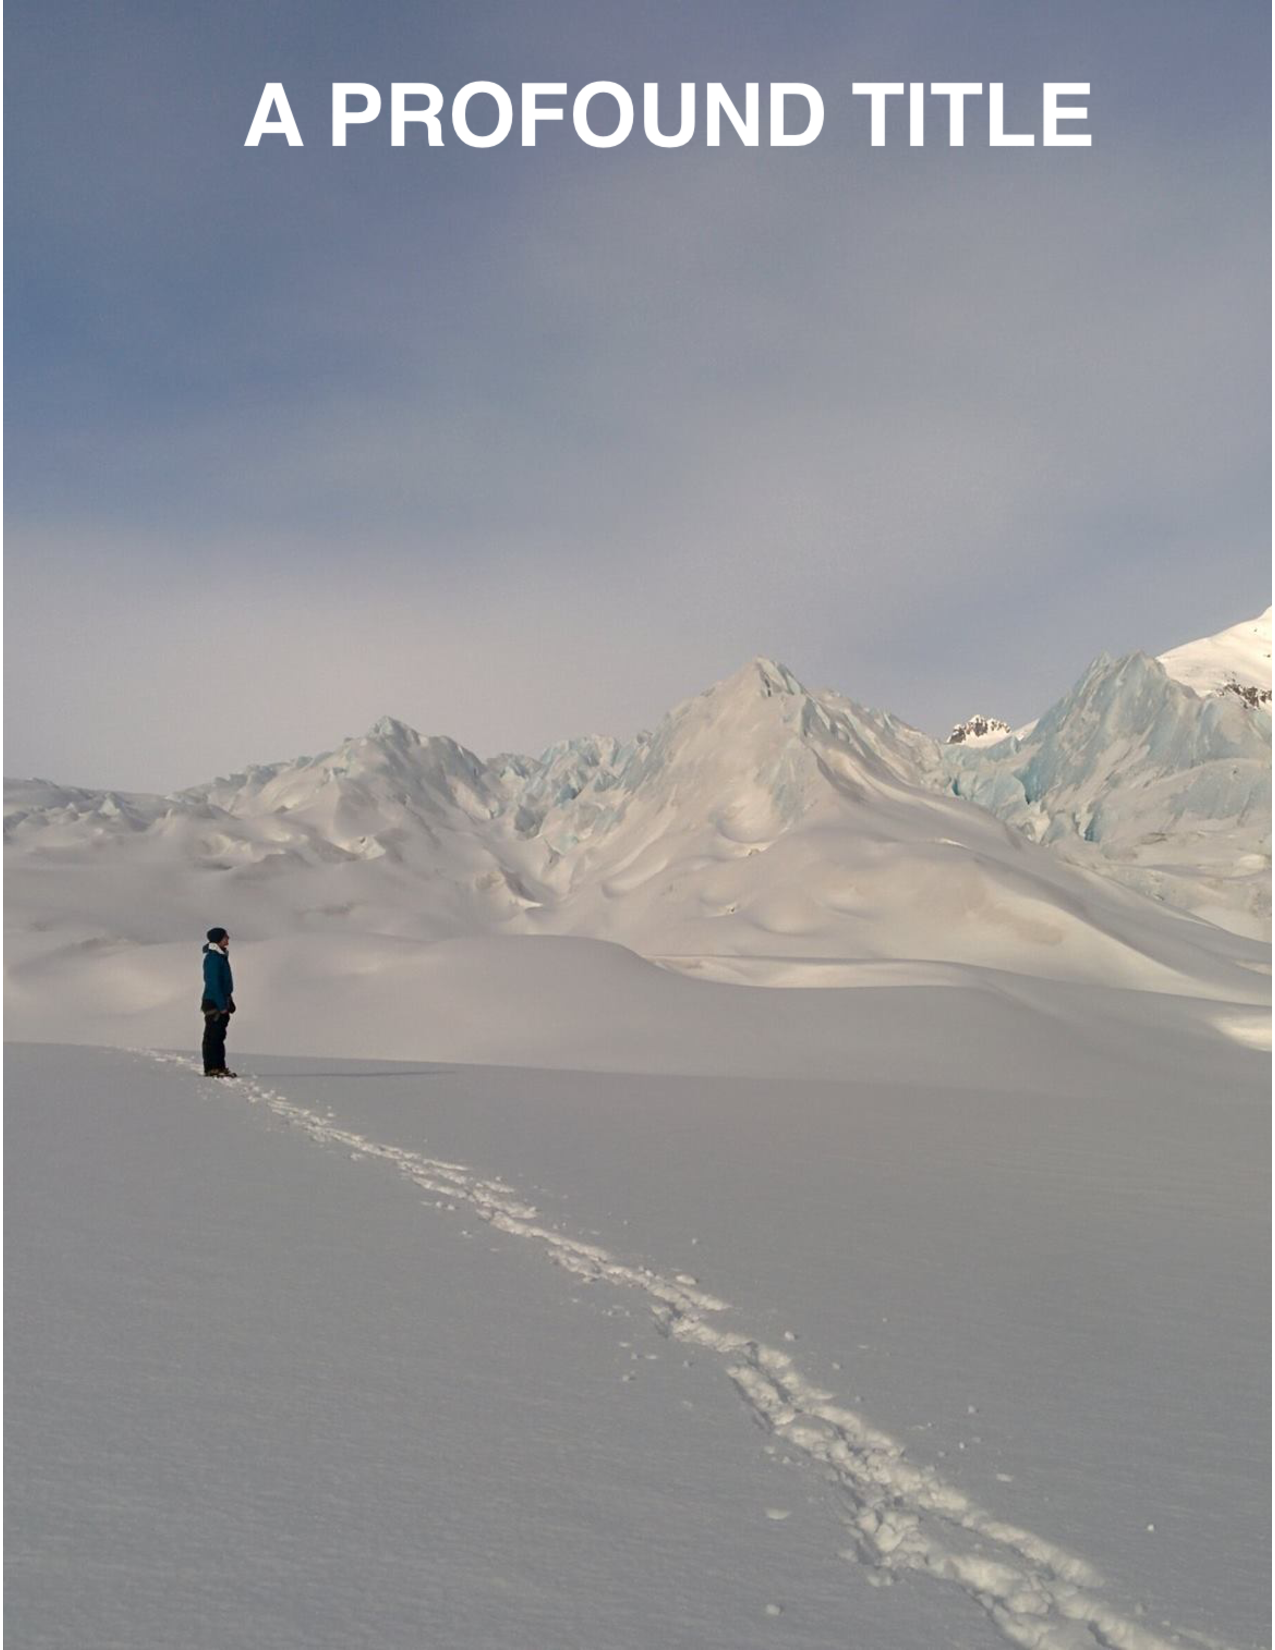
\includepdf[pages={1}]{book-cover.pdf}
% Title and copyright pages

\thispagestyle{empty}
\license
\vspace{1in}
\begin{center}
Edition\\
% Indicate if solutions are printed.
\vspace{0.5in}
\ifthenelse{\boolean{SOLUTIONS}}{\textbf{INSTRUCTOR SOLUTIONS EDITION}}{~}
\end{center}

\vfill

% Trademark notice
{\tiny HyperGlobalMegaCom\tm, PleaseDontSueMe\tm, and CanYouReallyTrademarkThis\tm are trademarks owned by HyperGlobalMegaCom, Inc.\\
Eclipse\tm is a trademark owned by The Eclipse Foundation.

All other trademarks, service marks, and trade names referenced in this text are the property of their respective owners.

Unless otherwise noted, this text has no association with any other company, product, or trademark.} 


% Table of contents
\clearpage
\begin{spacing}{0.0}        % More compact table of contents
\markboth{CONTENTS}{}
\setcounter{tocdepth}{1}    % Normally, the depth of the TOC is 2, but this makes the TOC very long.
\tableofcontents
\end{spacing}
\addtocontents{toc}{\vspace{-0.5in}}

% preface
\clearpage
% Authors: Jeff C. Jensen, Edward A. Lee and Sanjit A. Seshia
% Date: 2016-06-08
% Copyright: (c) 2016, all rights reserved.
% License: Creative Commons Attribution 4.0 International (CC BY 4.0).

% \chapter* is an unnumbered chapter, and will appear in index and TOC.
\chapter*{Preface}\label{chap:preface}
% \markboth sets header, such as chapter title and page number
\markboth{PREFACE}{}
% this is where the TOC will appear
\addcontentsline{toc}{chapter}{Preface}

% \section* is an unnumbered section, and will appear in index and TOC.
\section*{What this Book is About}
... and it had better be good.

\section*{Intended Audience}
... and they had better be eager to learn.

\section*{Acknowledgements}
... because you probably didn't do this alone.


%%%%%%%%%%%%%%%
% Main Matter
%%%%%%%%%%%%%%%
\clearpage
% ahead there be dragons, this is the informational content of the book
\mainmatter
\chapter{Topic 1}\label{chap:topic1}

%%%%%%%%%%%%%%%%%%%%%%%%%%%%%%%%%%
%     Introduction               %
%%%%%%%%%%%%%%%%%%%%%%%%%%%%%%%%%%
\section{Introduction}\label{sec:topic1-introduction}
Lay down the theory. G{\"o}del shows whatever theory you have to lay down, it has zero measure in the grand scheme of things. So be humble.

\subsection{Definitions}\label{sec:topic1-introduction-definitions}
A definition of an \definition{alien} is a term described here, and automatically added to the index. A subtle difference is the \definition{Tralfamadore}, the definition of a proper noun which should be capitalized. In LaTeX the index term and its label may differ in capitalization, which can cause problems. This book makes the LaTeX label lowercase, and uses specicial definitions and links for the text to appear in lower or upper case. Use \textbackslash definition or \textbackslash Definition to define. Links to previously defined references are similarly handled by \textbackslash definitionlink and \textbackslash Definitionlink to appear in lower and upper case, respectively. There is a better solution for this, but I haven't room in the margin for the code snippet.

A bothersome term to define is an ancronym such as \acronym{three-leter acronym}{TLA}, for which you would like both the abbreviation and the expanded term to appear in the index with an appropriate link. Look for the term in the index, and try following the definition link which should bring you to the beginning of the paragraph in which it is defined: \definitionlink{TLA}.

\subsection{Filler}\label{sec:topic1-introduction-filler}
Lorem ipsum dolor sit amet, consectetur adipiscing elit. Ut a porttitor elit. Integer sem dolor, egestas eu auctor ut, suscipit quis lorem. Sed nisi augue, euismod non massa sit amet, pellentesque fringilla elit. Phasellus et fringilla erat. Praesent gravida ullamcorper nunc nec feugiat. Etiam dapibus finibus ante, in molestie augue interdum vitae. Quisque non feugiat diam. Nam commodo mattis ante in ullamcorper. Integer euismod porttitor rhoncus. Aenean eget imperdiet libero. Aliquam erat volutpat. Integer ut viverra augue. Quisque purus ante, pretium vel sapien ut, tincidunt laoreet massa.

Fusce a sapien egestas, placerat tellus vitae, sagittis metus. Sed vitae porttitor diam. Aenean ipsum nulla, iaculis et orci et, luctus interdum leo. Ut rhoncus luctus metus in sodales. Phasellus hendrerit neque nec magna viverra interdum. Pellentesque commodo pharetra magna, non consequat odio semper vitae. Ut elit purus, faucibus at diam eu, malesuada consectetur nunc. Maecenas lectus orci, finibus vitae arcu et, sagittis pellentesque sem. Pellentesque fringilla odio non augue tincidunt, non fermentum lacus luctus. Nam venenatis non nisi ut luctus. Fusce eu ligula augue. Pellentesque ut mauris nulla. Suspendisse faucibus vel odio ut congue. Vivamus orci nulla, convallis eu cursus ac, lacinia quis nunc. Nam at est ante. Fusce mollis rhoncus eros, id facilisis leo efficitur sit amet.

Etiam ut erat iaculis, sodales urna vitae, egestas eros. Maecenas efficitur, arcu eu varius bibendum, ante diam ultricies augue, pulvinar tincidunt nunc lorem dictum erat. Cras porta massa mauris, ut consectetur nisl posuere a. Quisque sit amet dapibus justo. In in neque ut ex finibus iaculis. Proin egestas quam at leo ornare scelerisque. Vestibulum blandit consectetur metus accumsan vestibulum. Morbi consequat lacinia tempus. Integer varius dolor a nisi mollis congue.

Pellentesque feugiat odio orci, quis eleifend dolor aliquet a. Ut et vestibulum tellus. Nunc venenatis ipsum id volutpat placerat. Pellentesque vitae semper arcu. Suspendisse sit amet tempor orci. Praesent venenatis lacinia luctus. Fusce auctor lectus fringilla sapien finibus aliquam. Etiam eget nisl hendrerit, vehicula magna ut, consequat velit. Donec eget urna ultrices, scelerisque libero eu, congue nisi. Mauris in feugiat metus, a ultricies libero. Aliquam tincidunt, eros ut porta dapibus, est nulla posuere risus, eu aliquam diam mauris nec ligula. Phasellus ac quam et lectus porttitor laoreet. Duis rhoncus massa a felis tincidunt, non dictum elit pellentesque. Vivamus dictum tempus vulputate. Nam accumsan urna non nibh rutrum, id sagittis urna placerat.

Integer varius, urna quis sagittis vulputate, orci lectus iaculis lorem, eu lacinia augue augue ut leo. Praesent augue mauris, sagittis sit amet fermentum a, aliquet ut purus. Curabitur quis libero velit. Vestibulum hendrerit, est in bibendum aliquet, elit ligula luctus lorem, non tempus eros ligula in eros. Duis ornare vulputate bibendum. Quisque sit amet interdum mauris. Mauris aliquam, tellus vel maximus maximus, nunc sapien placerat mauris, ut viverra ante lacus sit amet massa. Donec eget sem tincidunt, finibus enim a, ullamcorper orci. Integer molestie ex vitae dui dapibus, id dignissim arcu luctus. Phasellus fringilla lacinia mauris a tincidunt. Phasellus vel pretium diam, a pharetra nisi. Sed ut eros mi. Ut tempor mi quam, at sagittis dui lobortis quis. Integer finibus neque non odio faucibus luctus.

Fusce sodales eu odio gravida bibendum. Proin sed leo ut risus fermentum consectetur. Suspendisse euismod posuere nulla, ac semper libero vulputate eu. Nam aliquet erat non urna fermentum, non semper nulla iaculis. Nunc ornare lorem ac ornare dictum. Nunc commodo mi et mattis fermentum. Donec faucibus nisi ut dolor tempus mattis. Nam congue sapien vel tellus congue congue. Maecenas quis lacus sit amet nisl commodo volutpat ac non neque. Proin ac sollicitudin justo. Aliquam erat volutpat. Suspendisse nec mattis urna.

\clearpage
% Authors: Jeff C. Jensen, Edward A. Lee and Sanjit A. Seshia
% Date: 2016-06-08
% Copyright: (c) 2016, all rights reserved.
% License: Creative Commons Attribution 4.0 International (CC BY 4.0).

\chapter{Topic 2}\label{chap:topic2}

\section{Introduction}\label{sec:topic2}
This topic includes figures and exercises.

%%%%%%%%%%%%%%%%%%%%%%%%%%%%%%%%%
%          EXERCISES            %
%%%%%%%%%%%%%%%%%%%%%%%%%%%%%%%%%
\section{Topic 2 Exercises}\label{sec:topic2-exercises}
A few example exercises. Note that solutions appear only if \textbackslash SOLUTIONS is set to true in book.tex.

\begin{asparaenum}
\item Why do grocery stores sell hot dogs in packs of 10 and hot dog buns in packs of 8?

    \begin{solution}
        It's a conspiracy.
    \end{solution}

\item Let $\vec{a}_g=(a_{g_x},a_{g_y},a_{g_z})$ be the specific force of gravity as measured by an accelerometer on a mobile robot. You may assume the accelerometer has been calibrated and is in units of g.
    \begin{compactenum}
    \item Find $\vec{a}_g$ when the robot is on level ground. Verify $\norm{\vec{a}_g}=1g$.
        \begin{solution}
        \begin{equation*}
        \vec{a}_g = 1g\begin{bmatrix}
            0 \\
            0 \\
            1
            \end{bmatrix}
        \end{equation*}

        \begin{equation*}
        \begin{aligned}
        \norm{\vec{a}_g}&=1g\sqrt{0^2+0^2+1^2} \\
        &=1g
        \end{aligned}
        \end{equation*}
        \end{solution}

    \item The robot is placed on a hill with inclination $\theta_\text{I}\in\left[0,\tfrac{\pi}{2}\right]$ in radians. Find $\vec{a}_g$ when the robot is oriented directly uphill. Verify $\norm{\vec{a}_g}=1g$.
        \begin{solution}
        \begin{equation*}
        \vec{a}_g=1g
            \begin{bmatrix}
            \sin(\theta_\text{I}) \\
            0 \\
            \cos(\theta_\text{I})
            \end{bmatrix}
        \end{equation*}

        \begin{equation*}
        \begin{aligned}
        \norm{\vec{a}_g}&= 1g\sqrt{\sin^2(\theta_\text{I})+0^2+\cos^2(\theta_\text{I})}
        \\ &= 1g
        \end{aligned}
        \end{equation*}
        \end{solution}

    \item The robot is placed on a hill with inclination $\theta_\text{I}\in\left[0,\tfrac{\pi}{2}\right]$ in radians. Find $\vec{a}_g$ when the robot is rotated $\theta$ radians clockwise from uphill orientation. Verify $\norm{\vec{a}_g}=1g$.
        \begin{solution}
        \begin{equation*}
        \vec{a}_g=1g\begin{bmatrix}
            \sin(\theta_\text{I})\cos(\theta) \\
            \sin(\theta_\text{I})\sin(\theta) \\
            \cos(\theta_\text{I})
            \end{bmatrix}
        \end{equation*}

        \begin{equation*}
        \begin{aligned}
        \norm{\vec{a}_g}&=1g\sqrt{\sin^2(\theta_\text{I})\cos^2(\theta)+\sin^2(\theta_\text{I})\sin^2(\theta)+\cos^2(\theta_\text{I})} \\ &= 1g\sqrt{\sin^2(\theta_\text{I})\left[\cos^2(\theta)+\sin^2(\theta)\right]+\cos^2(\theta_\text{I})} \\ &= 1g\sqrt{\sin^2(\theta_\text{I})+\cos^2(\theta_\text{I})} \\ &= 1g
        \end{aligned}
        \end{equation*}
        \end{solution}
    \end{compactenum}
\end{asparaenum}


%%%%%%%%%%%%%%%%%%%%%%%%%%%%%%%%%%
%     WiiMote                    %
%%%%%%%%%%%%%%%%%%%%%%%%%%%%%%%%%%
\section{Introducing the WiiMote}\label{sec:topic2-wiimote}
This section shows various types of references, including references within this document, to an external website, and to an exernal PDF (remote or on disk).

%%%%%%%%%%%%%%%%%%%%%%%%%%%%%%%%%%%%%%%
%          PRELAB READING             %
%%%%%%%%%%%%%%%%%%%%%%%%%%%%%%%%%%%%%%%
\subsection{Prelab Reading}
\begin{compactitem}
\item \secref{sec:topic2-wiimote}
\item \linkref{wiki:Wii_Remote}
\item \linkref{WiiBrew:12:WiiMote}
\item \docref{BluetoothSpecialInterestGroup:03:BluetoothHIDProfile}
    \begin{compactitem}
        \item \docpageref{BluetoothSpecialInterestGroup:03:BluetoothHIDProfile}{18}{\S ``Introduction to the HID Protocol''}, p. 18-23
        \item \docpageref{BluetoothSpecialInterestGroup:03:BluetoothHIDProfile}{57}{\S ``BT HID Transaction Header''}, p. 57-64
    \end{compactitem}
\item \docref{Fisher:10:UsingAnAccelerometerForInclinationSensing}
\item \docref{Ozyagcilar:11:ImplementingCompass}
\end{compactitem}


%%%%%%%%%%%%%%%%%%%%%%%%%%%%%%%%%%%%%%%
%          LAB PROCEDURE              %
%%%%%%%%%%%%%%%%%%%%%%%%%%%%%%%%%%%%%%%
\subsection{Lab Exercises}
This is an example of laboratory exercises using a Nintendo WiiMote.

Required equipment:
\begin{compactitem}
\item Nintendo Wii Remote
\end{compactitem}

\begin{asparaenum}
\item \textbf{Plot the uncalibrated accelerometer signal from the WiiMote:} after pairing, open and run \consoleinline{WiiMote Interface.exe}.

    \begin{compactenum}
    \item What are the values of the x and y axes when the WiiMote is at rest on level ground?
        \begin{solution}
        This will vary from device to device, and the grade on which the WiiMote rests, but 0g should produce output around 128 ADC units.
        \end{solution}

    \item What is the value of the z axis when the WiiMote is at rest on level ground? What quantity is being measured?
        \begin{solution}
        This will vary from device to device. At rest the z axis should produce output around 155 ADC units. This is a measurement of gravity, 1g.
        \end{solution}
    \end{compactenum}

\item \textbf{Measure sensitivity and bias of the accelerometer:} Using the signal plots, determine the sensitivity and bias of the sensor.

    \hint{Will it help to measure one of these quantities first before measuring the second?}

    \begin{compactenum}
    \item What bias did you record?
        \begin{solution}
        The bias of the accelerometer is typically around 128 ADC units.
        \end{solution}

    \item What sensitivity did you record?
        \begin{solution}
        The sensitivity of the WiiMote accelerometer is typically around 25 ADC units per g. A common mistake is to measure sensitivity without compensating for the bias, which produces an (incorrect) sensitivity around 25 + 128 ADC units. The accelerometer will not properly scale to $\pm 1g$ if this error is made.
        \end{solution}
    \end{compactenum}

    \item Provide the relevant MATLAB code and screenshots of changes (if any) to the block diagram.
        \begin{solution}
        The MATLAB code that performs the above calibration equation follows.

\begin{lstlisting}[language=matlab]
% calibrate to units of g-forces (g)
acceleration = (sensor - bias) ./ sensivity;

% magnitude (in g)
mag = norm(acceleration);
\end{lstlisting}
        \end{solution}

\item \textbf{Measure Pitch and Roll:} Measure the pitch and roll of the WiiMote.

    \begin{compactenum}
    \item What equations did you use to calculate pitch and roll?
        \begin{solution}
        The solution follows from \cite{Ozyagcilar:11:ImplementingCompass}, Eqn. 13 and Eqn. 15, where $G_{px}$ and $G_{py}$ are swapped. Given acceleration $\vec{s}=(s_x,s_y,s_z)\in\reals^3$,
        \begin{equation*}
        \begin{aligned}
        \text{roll}\triangleq\phi&=\tan^{-1}\left(\frac{s_x}{s_z}\right) \\
        \text{pitch}\triangleq\theta&=\tan^{-1}\left(\frac{-s_y}{s_x\sin(\phi)+s_z\cos(\phi)}\right)
        \end{aligned}
        \end{equation*}
        \end{solution}
    \end{compactenum}
\end{asparaenum}



\section{Figures}\label{sec:topic2-figures}
Here is the logo for the \pointer{GNU} project.

%fig:gnu
\begin{figure}[h]
\centering

\includegraphics[width=0.25\linewidth]{fig/gnu.png}
\figcaption{GNU logo~\cite[]{Suvasa:11:gnulogo}.\label{fig:gnu}}
\end{figure}


\section{Other Useful Definitions}
For inline code, such as \code{[]->int\{return 42;\}} use \textbackslash code .

For long file paths, such as
    \begin{longpath}
    /usr/bin/which
    \end{longpath}
use the \code{longpath} environment.

For a textual representation of a button, use \textbackslash dialogbutton . \dialogbutton{OK}

If you need to fix something in a future version, use \textbackslash fixme. It will show up if \textbackslash DRAFT is set to true in the preamble, and will be hidden otherwise. \fixme{Remind folks that this feature will change layout when text is hidden or shown.}

For a sequence of steps, such as navigating multiple menu levels, use \textbackslash menulist with items separated by colons:
\menulist{File:Import:Document}

For entering commands in a console, use \textbackslash consoleinline or the console environment.
\begin{console}
cd\\
sudo apt-get update\\
sudo apt-get upgrade\\
\end{console}


For code sections, use \textbackslash lstlisting. Default settings are set in the preable.
\begin{lstlisting}
#include <stdio.h>

int main(int argc, char **argv)
{
    printf("Hello, world!\n");
    return 0;
}\end{lstlisting}

% appendix
\clearpage
\appendix
\chapter{Appendix}\label{chap:Appendix}

%%%%%%%%%%%%%%%%%%%%%%%%%%%%%%
%     Appendix               %
%%%%%%%%%%%%%%%%%%%%%%%%%%%%%%
\section{Introduction}\label{sec:appendix-introduction}
Additional stuff goes here. Note that the placement of this chapter in book.tex uses letters instead of numbers for chapter index.


%%%%%%%%%%%%%%%
% Back Matter
%%%%%%%%%%%%%%%
\clearpage
\backmatter

\fancyfoot[L]{} % drop section footer

% Bibliography
% Use phantom section to ensure that the TOC bibliography goes to the right page:
\phantomsection
\addcontentsline{toc}{chapter}{Bibliography}
\fancyhead[L]{\slshape BIBLIOGRAPHY}
\bibliographystyle{jponewurl}
{\footnotesize
\bibliography{references,\referencesexternal}
}
\vfill
\clearpage

% Detailed table of contents
% Use phantom section to ensure that the TOC chapter link goes to the right page:
%\fancyhead[L]{\slshape \leftmark}
\phantomsection
\addcontentsline{toc}{chapter}{Index}
\fancyhead[L]{\slshape INDEX}
{\footnotesize
\printindex
}
\vfill

% Final quote
\clearpage
\fancyhf{}
\fancyfoot[R]{\thepage}
\vspace*{\fill}
\begin{center}
\begin{quote}
{\footnotesize Any final words?}
\end{quote}
\end{center}
\vspace*{\fill}

\end{document}

% Let it be known that LaTeX is the damned worst language on Earth.
